% Generated by analysis/18_wing_gallery.py. Do not edit by hand.
\section{The best delivered wings}
\label{app:gallery}

This appendix shows the best wing each method delivered. For the five baseline optimizers, we took the recommendation each method made after 32 queries in each of its ten episodes per task and kept the delivered one with the highest $L/D$. The open-ended research agent made no further requested checkpoint recommendation after query 4, so for it we took the delivered online design with the highest $L/D$ among queries 5 to 32 of its 30 extension episodes. Figure~\ref{fig:wing-gallery} draws the 16 wings at one scale, and Table~\ref{tab:wing-gallery} lists their planform values. CMA-ES with no feedback and CMA-ES with selection only each delivered no recommendation after 32 queries at $C_L=0.15$, so those two cells are empty. CMA-ES with no feedback and CMA-ES with selection only delivered the same wing at $C_L=0.66$. The best wings of the different methods are all thin and swept, with a high aspect ratio. Their leading-edge sweep ranges from 26 to 44 degrees, their aspect ratio from 8.9 to 12.5, their taper ratio from 0.26 to 0.52, and their root thickness ratio from 0.126 to 0.138. The highest score at each load is 19.31 for open-ended research at $C_L=0.15$, 34.05 for open-ended research at $C_L=0.41$ and 32.37 for feedback-guided CMA-ES at $C_L=0.66$. Every wing shown was delivered by the CFD evaluator, so each score is a graded result rather than a surrogate prediction.

\begin{figure}[H]
\centering
% Natural size keeps every wing at its printed size; see
% analysis/18_wing_gallery.py.
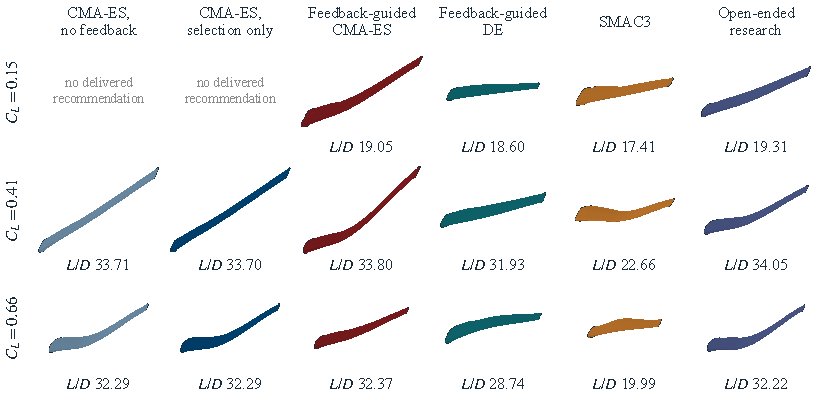
\includegraphics{fig_wing_gallery.pdf}
\caption{The best delivered wing of each method and task, drawn as in Figure~\ref{fig:wing-mesh-outcomes} at one scale. For the five baselines it is the delivered recommendation after 32 queries with the highest $L/D$ over the ten seeds. For open-ended research it is the delivered online design with the highest $L/D$ among queries 5 to 32 of its 30 extension episodes. Each number is the wing's $L/D$. The two archive-only CMA-ES methods delivered nothing after 32 queries at $C_L=0.15$, so those cells are empty.}
\label{fig:wing-gallery}
\end{figure}

\begin{table}[H]
\caption{The wings of Figure~\ref{fig:wing-gallery}. Seed is the episode seed, and for open-ended research the episode label. Sweep is the leading-edge sweep in degrees, taper ratio is the tip chord over the root chord, and root $t/c$ is the thickness of the root section over its chord. The four are columns 0, 3, 4 and 37 of the 38 design variables, in the order of the released tables and the guide, and they are the planform values the guide defines without an interpolation rule. A dash marks a cell with no delivery.}
\label{tab:wing-gallery}
\centering
\scriptsize
\setlength{\tabcolsep}{4pt}
\begin{tabular*}{\textwidth}{@{\extracolsep{\fill}}llrrrrrr}
\toprule
method & $C_L$ & seed & $L/D$ & sweep ($^\circ$) & aspect ratio & taper ratio & root $t/c$ \\
\midrule
CMA-ES, no feedback & $0.15$ & -- & -- & -- & -- & -- & -- \\
 & $0.41$ & 6206 & 33.71 & 39.9 & 12.49 & 0.524 & 0.126 \\
 & $0.66$ & 6208 & 32.29 & 37.7 & 12.49 & 0.311 & 0.127 \\
CMA-ES, selection only & $0.15$ & -- & -- & -- & -- & -- & -- \\
 & $0.41$ & 6206 & 33.70 & 39.8 & 12.49 & 0.524 & 0.127 \\
 & $0.66$ & 6208 & 32.29 & 37.7 & 12.49 & 0.311 & 0.127 \\
Feedback-guided CMA-ES & $0.15$ & 6202 & 19.05 & 43.6 & 12.27 & 0.524 & 0.138 \\
 & $0.41$ & 6201 & 33.80 & 37.1 & 12.49 & 0.524 & 0.126 \\
 & $0.66$ & 6209 & 32.37 & 36.1 & 12.49 & 0.272 & 0.126 \\
Feedback-guided DE & $0.15$ & 6207 & 18.60 & 40.9 & 11.87 & 0.257 & 0.130 \\
 & $0.41$ & 6203 & 31.93 & 37.8 & 12.32 & 0.407 & 0.131 \\
 & $0.66$ & 6204 & 28.74 & 38.9 & 12.15 & 0.292 & 0.128 \\
SMAC3 & $0.15$ & 6202 & 17.41 & 39.8 & 10.54 & 0.475 & 0.129 \\
 & $0.41$ & 6202 & 22.66 & 26.1 & 11.74 & 0.524 & 0.126 \\
 & $0.66$ & 6204 & 19.99 & 36.7 & 8.90 & 0.356 & 0.135 \\
Open-ended research & $0.15$ & 9531 & 19.31 & 39.5 & 11.52 & 0.524 & 0.128 \\
 & $0.41$ & 9551 & 34.05 & 39.3 & 12.45 & 0.357 & 0.131 \\
 & $0.66$ & 9531 & 32.22 & 39.0 & 12.46 & 0.283 & 0.133 \\
\bottomrule
\end{tabular*}
\end{table}
